% Figure 3 — selective signal vs base rate by test year (standalone, vector PDF).
\documentclass[border=3pt]{standalone}
\usepackage{tikz}
\usepackage{pgfplots}
\pgfplotsset{compat=1.17}
\begin{document}
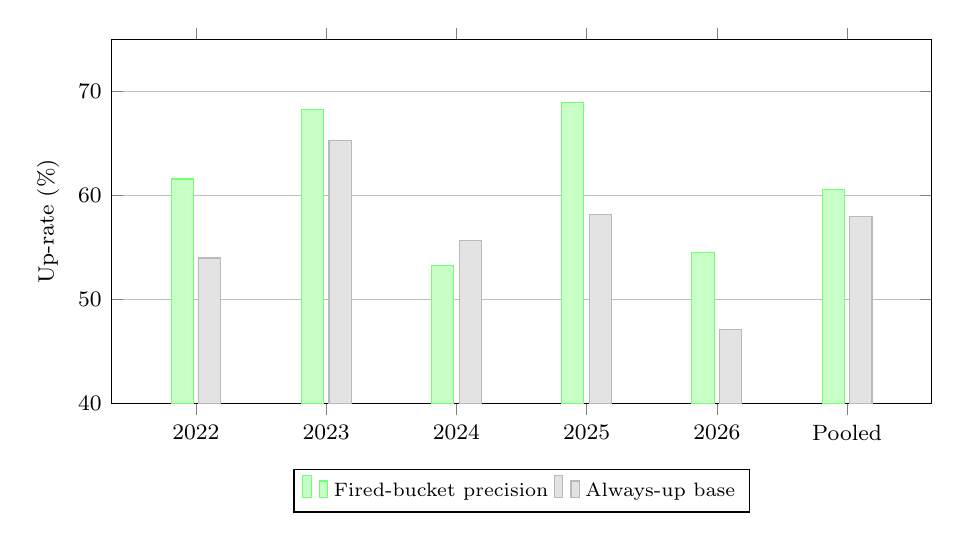
\begin{tikzpicture}
\begin{axis}[
  width=12cm, height=6.2cm, font=\footnotesize,
  ybar, bar width=8pt,
  symbolic x coords={2022,2023,2024,2025,2026,Pooled},
  xtick=data, ymin=40, ymax=75, ylabel={Up-rate (\%)},
  enlarge x limits=0.13, ymajorgrids,
  legend style={at={(0.5,-0.18)},anchor=north,legend columns=2,font=\scriptsize}
]
\addplot[fill=green!22,draw=green!55] coordinates {(2022,61.6)(2023,68.3)(2024,53.3)(2025,69.0)(2026,54.5)(Pooled,60.6)};
\addplot[fill=gray!22,draw=gray!55] coordinates {(2022,54.0)(2023,65.3)(2024,55.7)(2025,58.2)(2026,47.1)(Pooled,58.0)};
\legend{Fired-bucket precision, Always-up base}
\end{axis}
\end{tikzpicture}
\end{document}
